\chapter{System Design}
\label{chap:design}

\section{High-Level Architecture}
\label{sec:architecture}

The system is organised into four tiers, shown in Figure~\ref{fig:architecture}: a client tier
running in the browser, a delivery tier built on Amazon CloudFront, an application tier
comprising the backend API and the database, and a processing tier that performs transcoding.

\begin{figure}[H]
\centering
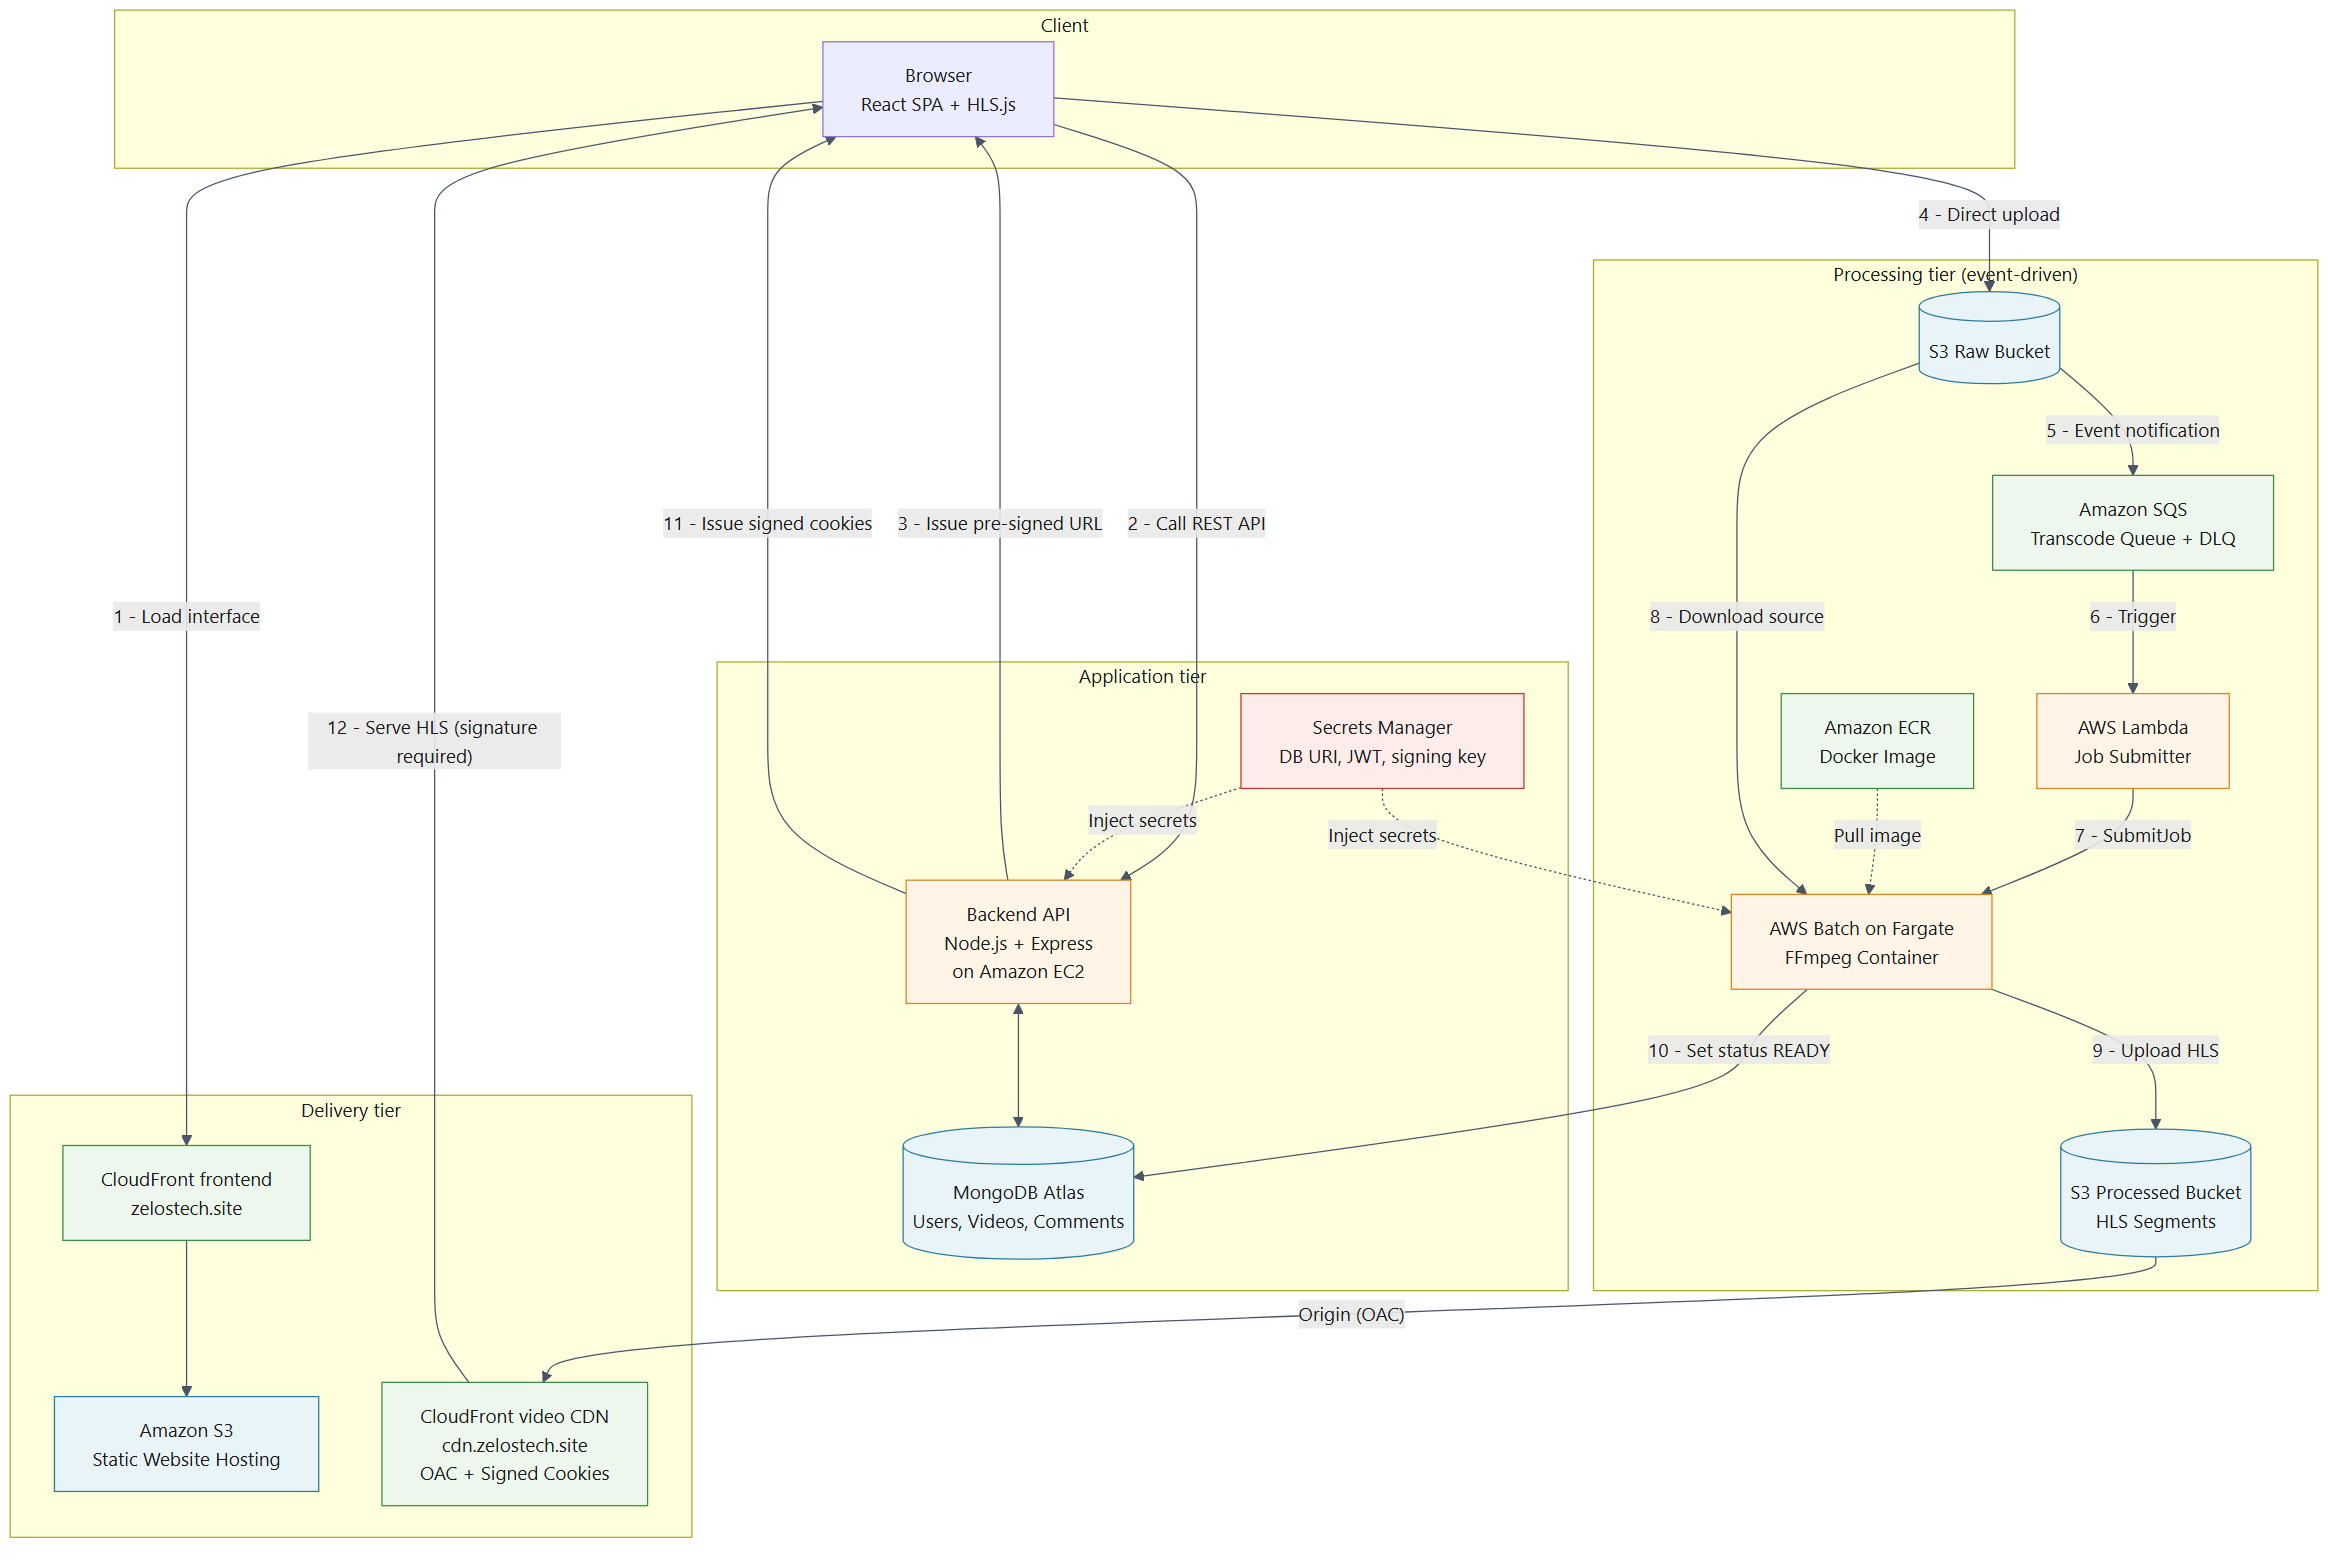
\includegraphics[width=\textwidth]{images/01-architecture-overview.png}
\caption{\textit{Overall system architecture and the eleven-step data flow}}
\label{fig:architecture}
\end{figure}

The separation between the application tier and the processing tier is the defining
characteristic of this design. The backend API never touches video content: it issues
pre-signed URLs, records metadata, and answers queries, while every byte of video flows
directly between the browser, Amazon S3, and CloudFront. This separation has three consequences
that together justify the architecture. The API server's resource consumption becomes
independent of video size and upload concurrency. The processing tier can scale according to
transcoding demand without affecting the responsiveness of the interface. And a failure in the
processing tier degrades the system gracefully, leaving already-published videos playable while
newly uploaded ones remain in a pending state.

\section{Transcoding Pipeline Design}
\label{sec:pipeline-design}

Figure~\ref{fig:sequence} traces the sequence of interactions from the moment the user
initiates an upload until the video becomes available.

% Xoay ngang: so do nay rong 6792 px voi tam doi tuong, dat vua chieu rong
% vung chu thi nhan chi con khoang 3pt. Xoay ngang cho phep dung chieu cao
% trang lam chieu rong hinh, lon hon 54 phan tram.
\begin{sidewaysfigure}
\centering
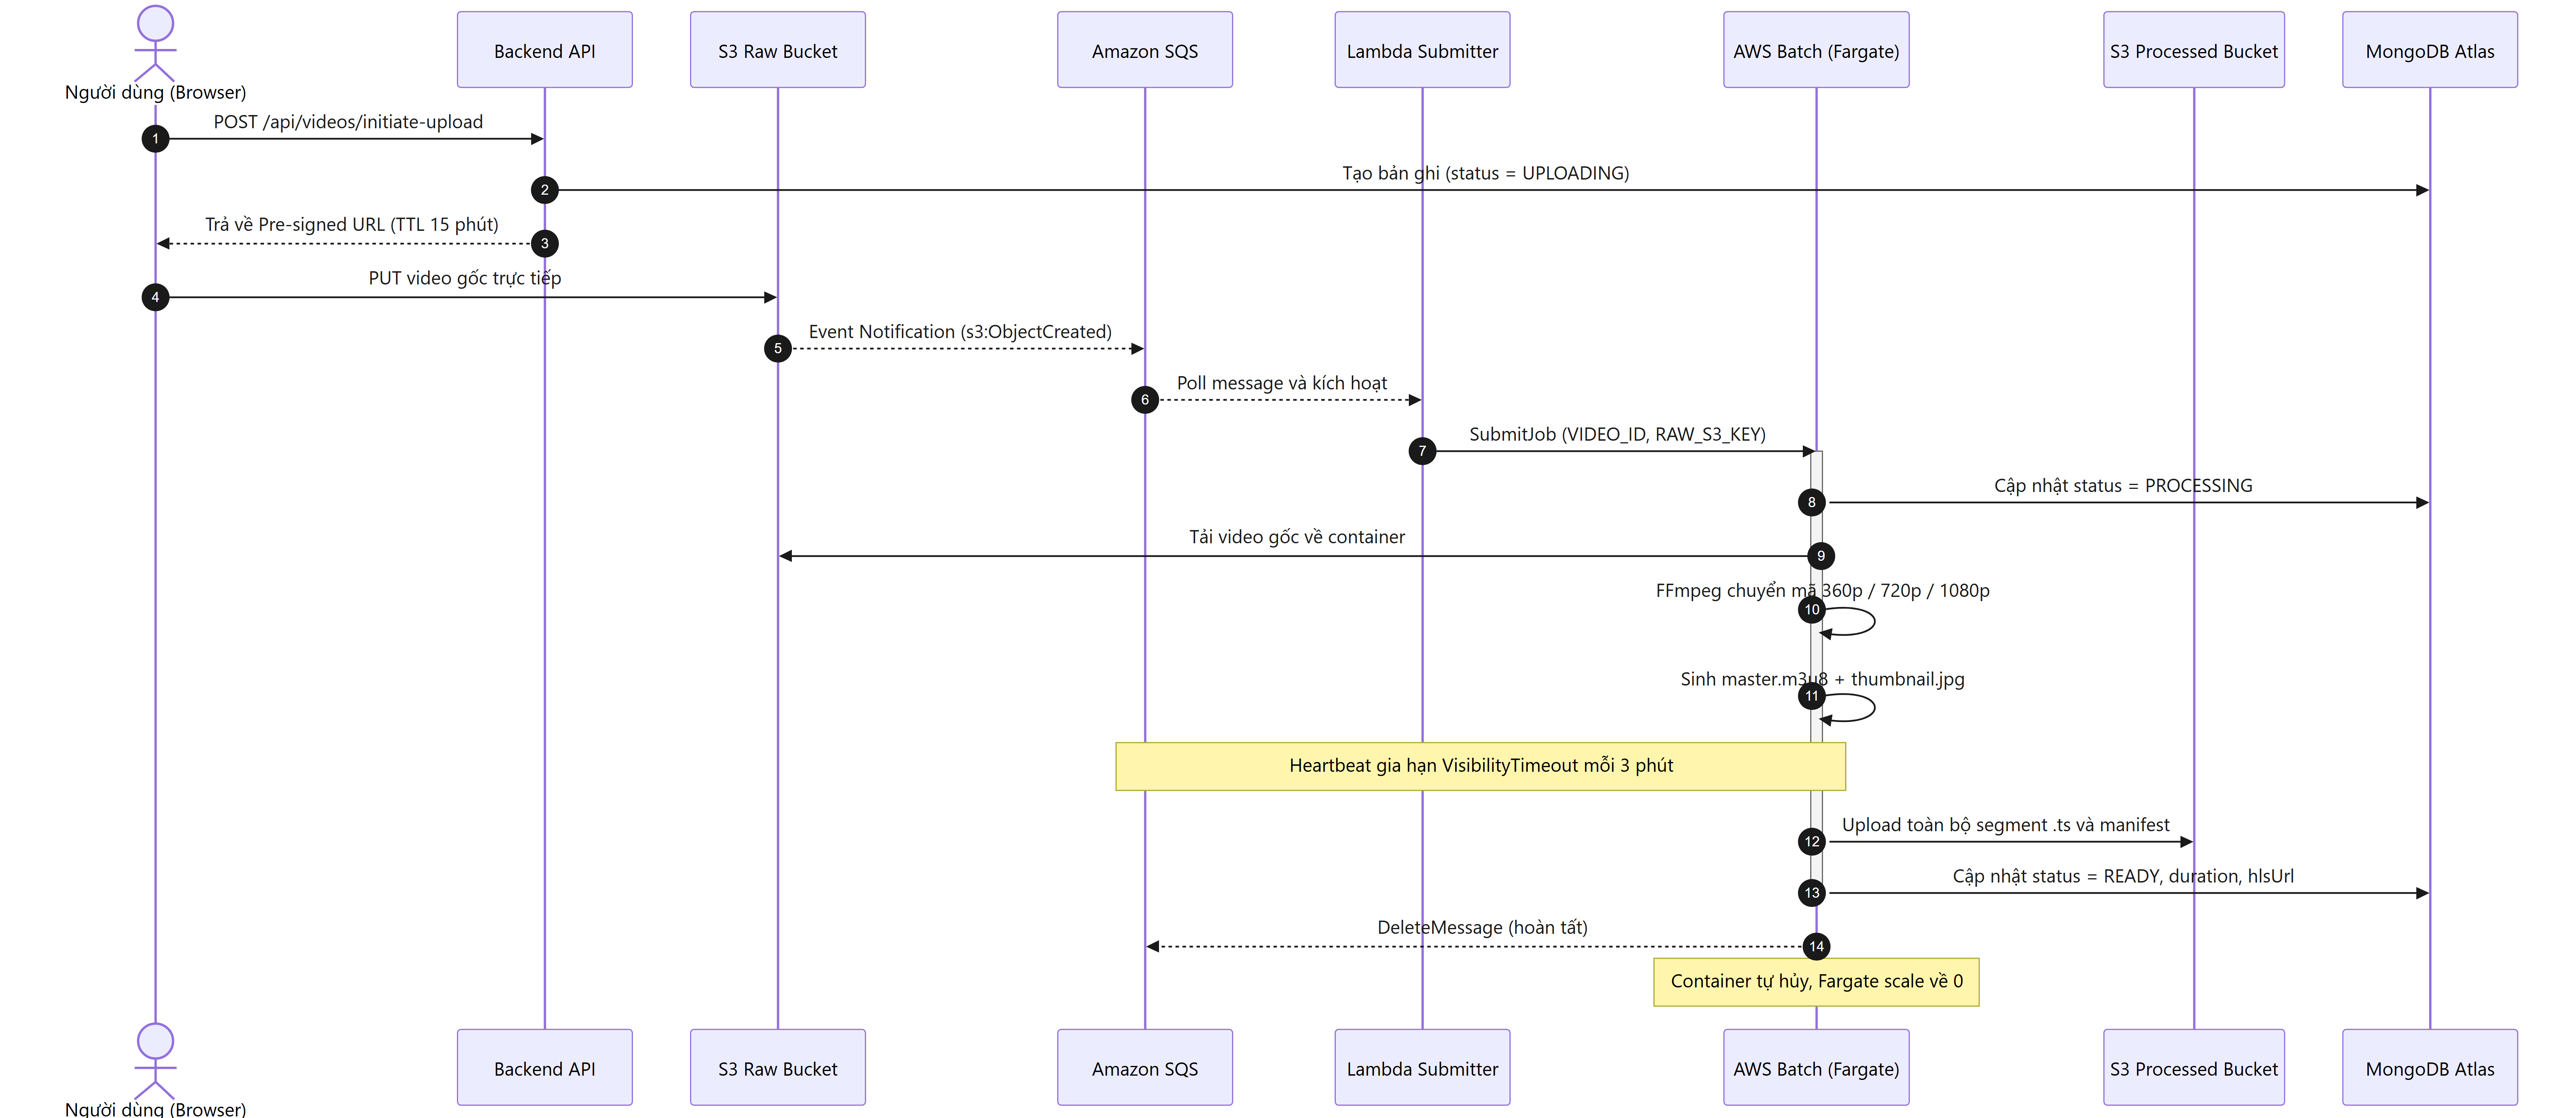
\includegraphics[width=\textheight]{images/02-transcoding-sequence.png}
\caption{\textit{Sequence diagram of the event-driven transcoding pipeline}}
\label{fig:sequence}
\end{sidewaysfigure}

Two design decisions embedded in this sequence merit explanation.

The first concerns the ordering of database record creation and URL issuance. The backend
creates the database record \emph{before} generating the pre-signed URL, and derives the S3
object key from the identifier of that record. The alternative, generating a key first and
creating the record afterwards, introduces a race condition: the S3 event notification can
arrive and trigger transcoding before the record exists, at which point the transcoder has no
row to update and the job fails. Creating the record first eliminates this class of failure
entirely.

The second concerns the visibility timeout of the SQS message. Amazon SQS hides a message from
other consumers for a configured period after it is received, and redelivers it if the consumer
has not deleted it by then. Transcoding a large file can easily exceed any reasonable fixed
timeout, which would cause the same video to be processed twice concurrently. The transcoder
therefore implements the heartbeat pattern: while FFmpeg runs, a timer periodically extends the
visibility timeout of the in-flight message. The message is deleted only after the job
completes successfully. If the container crashes, the heartbeat stops, the timeout lapses, and
the message returns to the queue for another attempt.

That description is accurate about the transcoder's \texttt{worker} mode, in which the container
consumes from the queue itself, but it is important to be precise that this is not the mode the
deployed system runs. The container image and the AWS Batch job definition both invoke
\texttt{batch} mode, in which the video identifier and object key arrive as environment variables
and the container never contacts SQS at all. The queue is consumed instead by the Lambda
submitter, which reads the message, submits a Batch job, and returns immediately. Because the
Lambda's work is finished at that point, the message is deleted when the job is \emph{submitted},
not when transcoding completes.

The consequence is that on the deployed path there is no heartbeat, and the message is long gone
before FFmpeg starts. Two properties the pattern was chosen to provide therefore have to be
obtained elsewhere. Protection against duplicate processing rests entirely on the conditional
database writes described in Section~\ref{sec:transcoder-impl}, which is where it belongs in any
case, since Burrows' analysis of leases (Section~\ref{sec:testing}) shows that a renewal timer
cannot by itself guarantee mutual exclusion. Retrying a failed job, which the heartbeat design
delegated to SQS redelivery, has no equivalent unless AWS Batch is configured to provide it; that
it originally was not is discussed in Section~\ref{sec:challenges}.

Retaining the worker-mode implementation is a deliberate choice rather than an oversight: it
allows the transcoder to be run against the queue directly during development without provisioning
Batch. Recording which of the two modes the evaluated system actually executes matters, though,
because a mechanism present in the source but absent from the deployed path cannot be credited
with the guarantees it would provide if it ran. Section~\ref{sec:challenges} draws the same
distinction about content protection.

\section{Database Design}
\label{sec:database-design}

The persistence layer uses MongoDB Atlas with three collections, shown in
Figure~\ref{fig:erd}.

\begin{figure}[htbp]
\centering
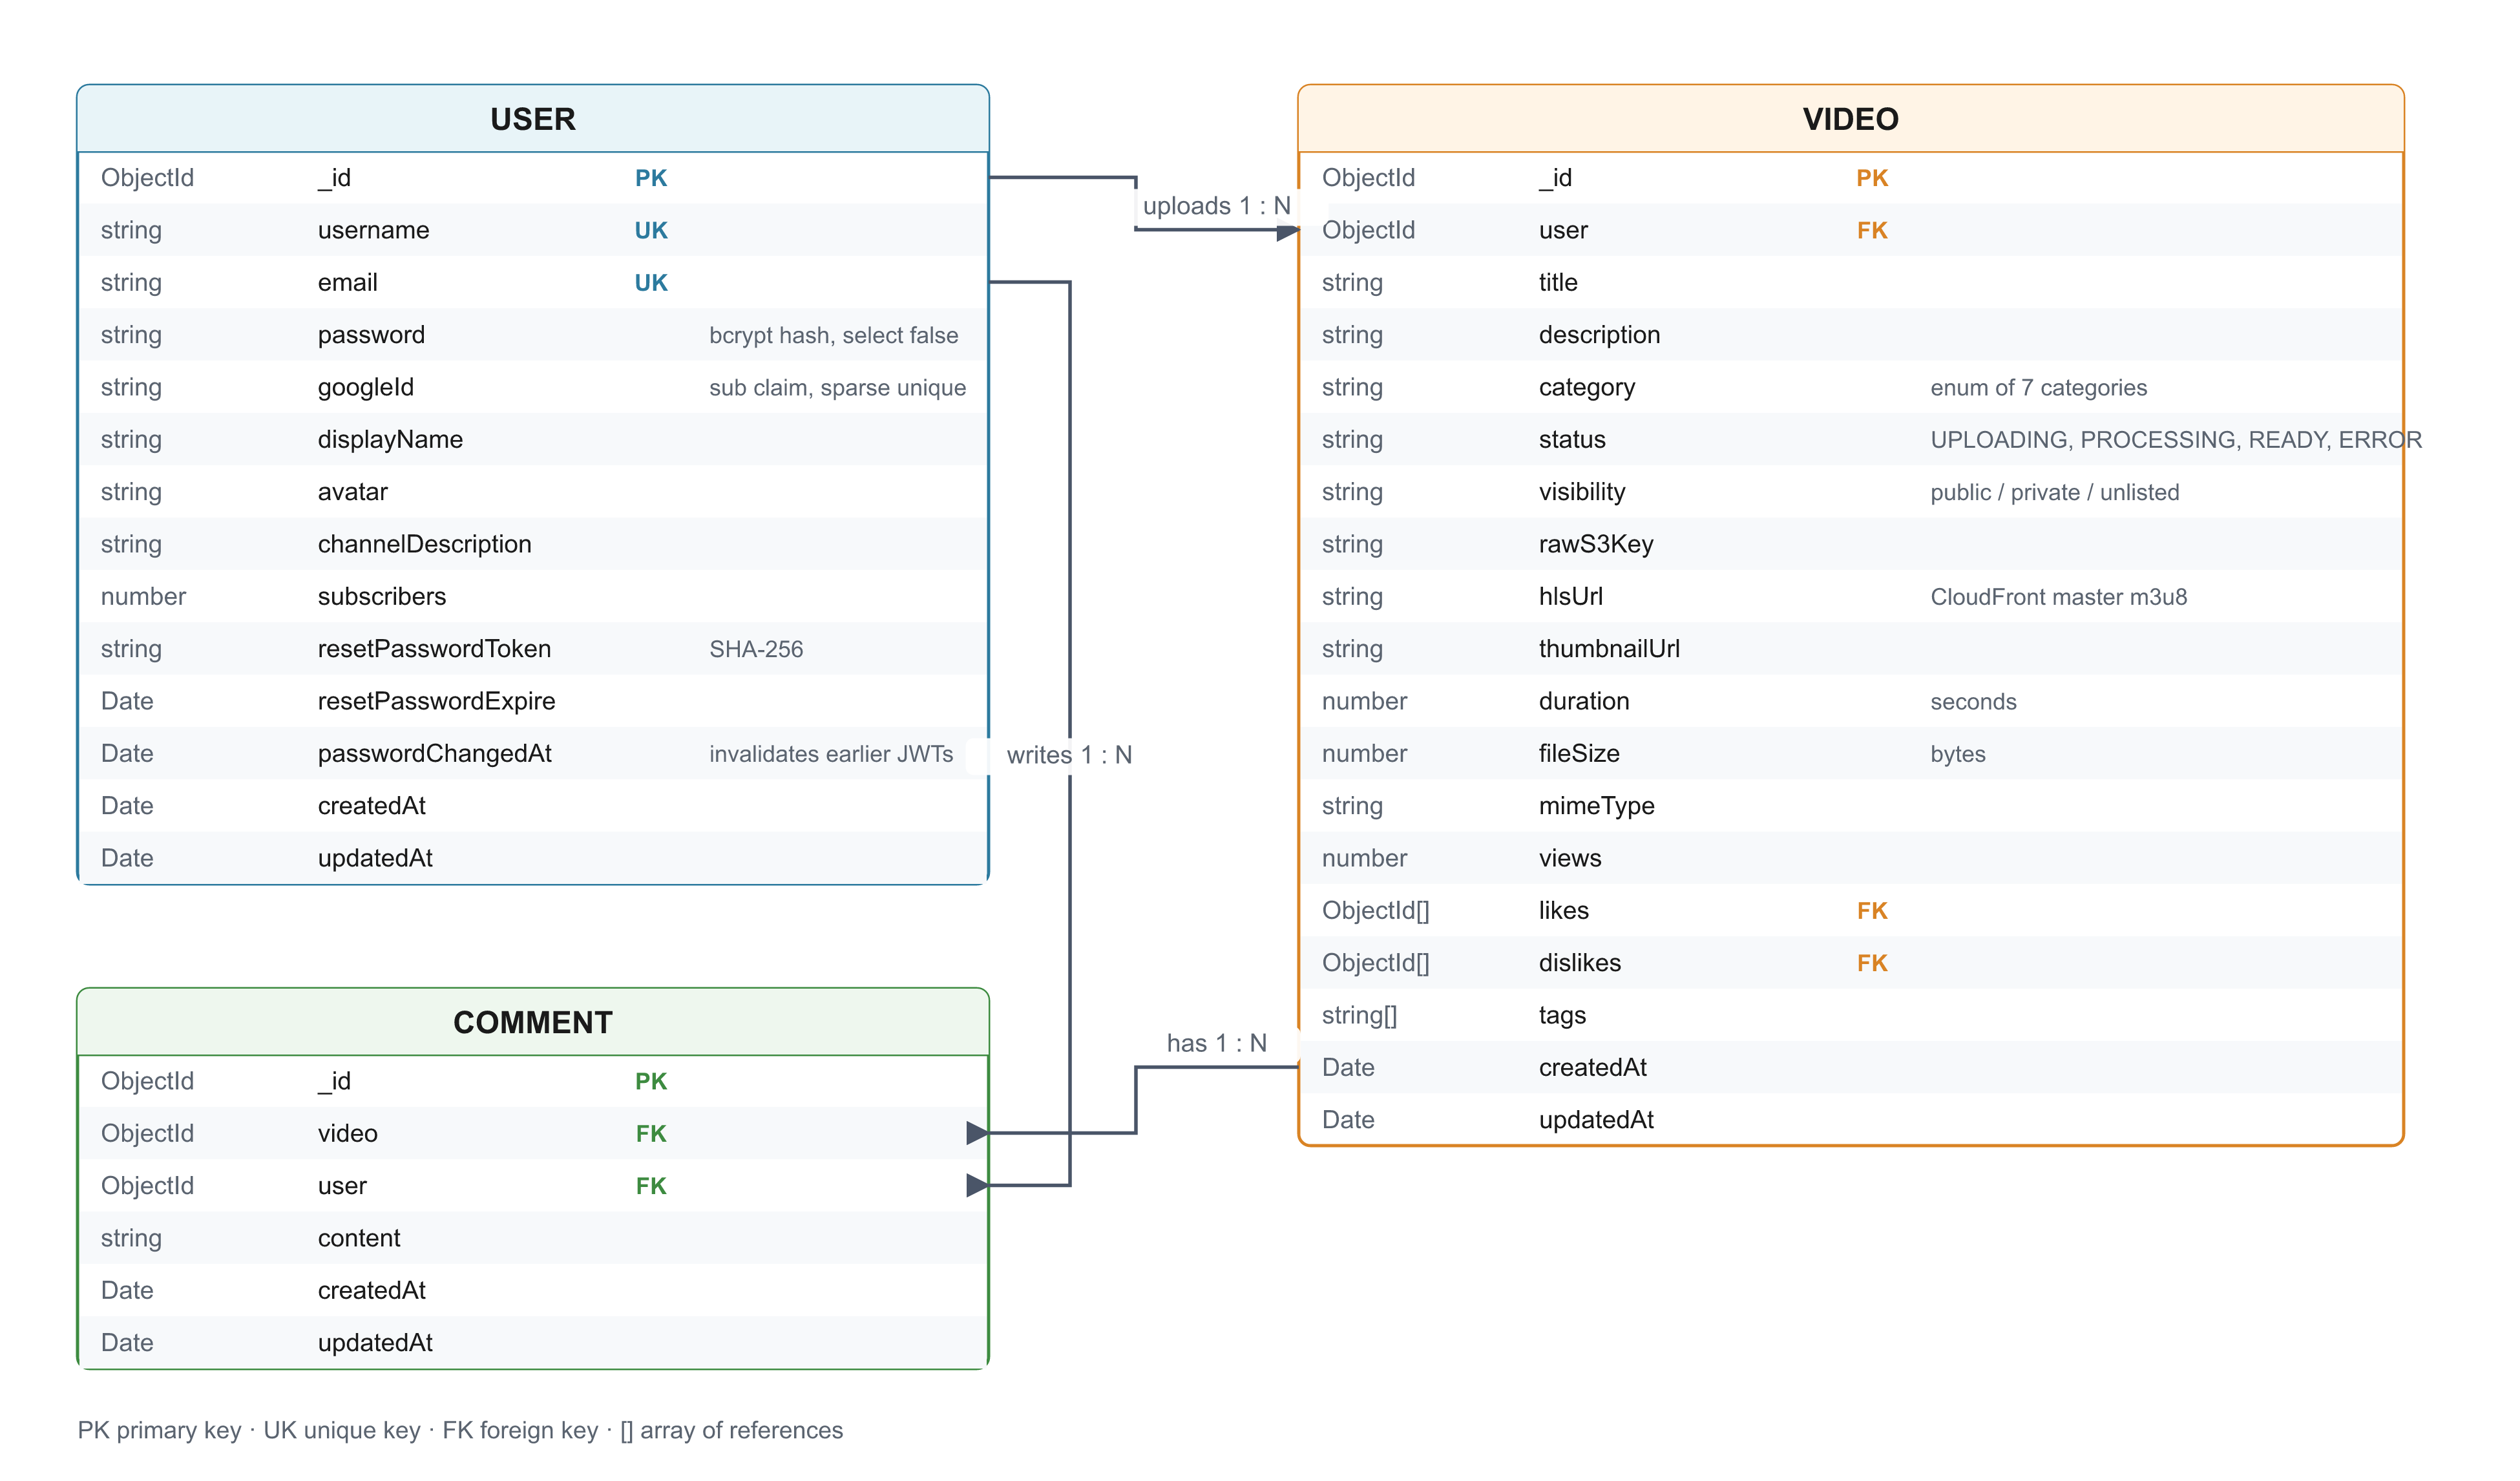
\includegraphics[width=\textwidth]{images/04-database-erd.png}
\caption{\textit{Entity relationship diagram of the MongoDB data model}}
\label{fig:erd}
\end{figure}

The \texttt{Video} document carries a \texttt{status} field that acts as a state machine with
four values. A record begins as \texttt{UPLOADING} when the pre-signed URL is issued, moves to
\texttt{PROCESSING} once the upload is confirmed and the job is submitted, and finally reaches
either \texttt{READY} or \texttt{ERROR}. Modelling the lifecycle explicitly rather than
inferring it from the presence of other fields makes the interface straightforward: the client
simply renders a different state for each value, and a video that failed to transcode is
distinguishable from one that is merely slow.

Likes and dislikes are stored as arrays of user identifiers embedded within the video document
rather than as a separate collection. The denormalisation is justified at this scale because the
counts are always read together with the video, and because a single user can appear at most once
in each array, so the arrays cannot grow through repeated interaction by the same person.

It should not be justified more strongly than that. Uniqueness bounds each array by the number of
distinct users, which is a bound only in the formal sense; on a widely viewed video it is exactly
the growth that a document store is poorly suited to hold, against MongoDB's document size limit.
The cost is also paid on reads that do not want it, since a listing of twelve videos retrieves
every identifier in all twenty-four arrays merely to display counts. The conventional remedy is a
separate collection with a compound unique index on video and user, plus a denormalised counter on
the video. That is the right structure for a system expecting popular content, and the reason it
was not adopted here is scale rather than principle. That is a different claim from the design
being correct in general, and it is recorded as such.

Indexes are defined to match the actual query patterns. A compound index on visibility, status,
and creation time supports the home page listing, which always filters on the first two fields
and sorts on the third.

Search is the exception. The collection carried a text index on title and description, described as supporting
the search feature, but no query ever used it: search is implemented as a case-insensitive regular
expression matched against title, description and tags, and MongoDB cannot serve an unanchored
regular expression from an index. Every search was a full collection scan, and the index cost
write throughput and storage while serving nothing. The index has been removed rather than the
query rewritten, because switching to a text search would change the feature's behaviour and not
merely its cost: the regular expression matches substrings inside words and covers the tags field,
neither of which a text index does. At the scale of this project a full scan is acceptable.

\section{Content Protection Design}
\label{sec:content-protection}

Protecting private content requires two complementary mechanisms, because each addresses a
different threat.

Origin Access Control makes the processed S3 bucket entirely private and grants read access
exclusively to the CloudFront distribution through a bucket policy. This prevents a viewer from
bypassing the content delivery network and fetching objects directly from S3, which would both
circumvent any access control implemented at the edge and incur higher data transfer charges.

Origin Access Control alone, however, does not determine \emph{who} may retrieve content
through CloudFront. Without a second mechanism, any person holding a manifest URL can download
the video regardless of its visibility setting, which would make the private mode ineffective
in practice. The system therefore adds CloudFront Signed Cookies backed by a trusted key group
\cite{awscloudfrontprivate}. The backend verifies the requester's permission using exactly the
same service function that governs the API response, signs a policy scoped to the directory of
that single video, and sets the resulting cookies on the response. CloudFront rejects any
request lacking a valid signature with HTTP 403 at the edge.

Signed cookies were chosen over signed URLs because of the structure of HLS. A playback session
retrieves a manifest and then hundreds of individual segment files, each as a separate request.
Signing each URL individually would require rewriting every entry inside the manifest,
typically using an edge function, which adds considerable complexity and cost. A single set of
cookies covers the entire directory and is attached automatically by the browser to every
subsequent request.

The policy is signed as a custom policy rather than a canned policy. This distinction is not
cosmetic: a canned policy does not permit wildcards in the resource path, whereas the required
scope is an entire directory. The custom policy expresses the resource as a pattern covering
the manifest and all segments of one specific video, which grants exactly the access needed and
no more.

One consequence of this design deserves stating precisely, because it is easy to describe the
scheme as protecting private videos and thereby understate it. The edge does not distinguish
public content from private: \emph{every} manifest and segment requires a valid signature, and a
request without one is refused whatever the video's visibility. What visibility governs is the
authorisation decision made earlier, when the backend decides whether to issue cookies at all.
Public and private videos are thus protected identically at the edge and differ only in who can
obtain the credential.

That uniformity has a limit that the design has to accommodate. A cookie authorises exactly one
video's directory, whereas a catalogue page renders thumbnails for many videos at once, and no
single cookie can cover them. Rather than weaken the policy scope to span the whole bucket, the
distribution carves out a separate cache behaviour for the thumbnail path that requires no
signature. The justification is that a thumbnail is not the asset the mechanism exists to
protect: it is a single low-resolution still, already shown to anyone permitted to see the video
in a listing, and treating it as public costs nothing that the scheme was designed to prevent.
The narrower point is that the protected unit is the stream, not every byte associated with a
video.

\section{Interface Design}
\label{sec:interface-design}

The frontend is a single page application composed of functional React components with hooks,
using React Context for authentication and theme state. Redux was considered unnecessary at
this scale, since the shared state consists only of the current user and the selected theme.

The video player is implemented as a custom component rather than relying on the browser's
native controls. The reason is that native controls cannot be extended: the browser renders its
own separate menu for playback speed and picture-in-picture, which cannot be merged with the
quality selector that HLS.js exposes. Presenting the user with two unrelated menus would be
confusing, so the component reimplements play and pause, seeking, volume, fullscreen, playback
speed, picture-in-picture, and rendition selection within a single settings menu.

The player also determines when a view is counted. Rather than incrementing the counter when
the page loads, which would allow the count to be inflated by repeated refreshes, the component
notifies the page only after playback has passed a threshold of several seconds, and the server
additionally ignores repeated reports from the same viewer within a thirty-minute window and
never counts the owner's own views.
